%%%%%%%%%%%%%%%%%%%%%%%%%%%%%%%%%%%%%%%%%%%%%%%%%%%%%%%%%%%%%%%%%%%%%%%%%%%%%%%
%                       CARGA DE LA CLASE DE DOCUMENTO                        %
%                                                                             %
% Las opciones admisibles son:                                                %
%      12pt / 11pt            (tamaño del cuerpo de letra; no usar 10pt)      %
%                                                                             %
% catalan/spanish/english     (idioma principal del trabajo)                  %
%                                                                             % 
% french/italian/german...    (si necesitáis usar otro idioma adicional)      %
%                                                                             %
% listoffigures               (El documento incluye un Índice de figuras)     %
% listoftables                (El documento incluye un Índice de tablas)      %
% listofquadres               (El documento incluye un Índice de cuadros)     %
% listofalgorithms            (El documento incluye un Índice de algoritmos)  %
%                                                                             %
%%%%%%%%%%%%%%%%%%%%%%%%%%%%%%%%%%%%%%%%%%%%%%%%%%%%%%%%%%%%%%%%%%%%%%%%%%%%%%%

\documentclass[11pt,spanish,listoffigures,listoftables]{tfgetsinf}

%%%%%%%%%%%%%%%%%%%%%%%%%%%%%%%%%%%%%%%%%%%%%%%%%%%%%%%%%%%%%%%%%%%%%%%%%%%%%%%
%                     CODIFICACIÓN DEL ARCHIVO FUENTE                         %
%                                                                             %
%    Windows suele usar 'ansinew'                                             %
%    en Linux es posible que sea 'latin1' o 'latin9'                          %
%    Pero lo más recomendable es usar utf8 (unicode 8)                        %
%                                          (si vuestro editor lo permite)     % 
%%%%%%%%%%%%%%%%%%%%%%%%%%%%%%%%%%%%%%%%%%%%%%%%%%%%%%%%%%%%%%%%%%%%%%%%%%%%%%%

\usepackage[utf8]{inputenc} 


%%%%%%%%%%%%%%%%%%%%%%%%%%%%%%%%%%%%%%%%%%%%%%%%%%%%%%%%%%%%%%%%%%%%%%%%%%%%%%%
%                       OTROS PAQUETES Y DEFINICIONES                         %
%                                                                             %
%%%%%%%%%%%%%%%%%%%%%%%%%%%%%%%%%%%%%%%%%%%%%%%%%%%%%%%%%%%%%%%%%%%%%%%%%%%%%%%

\usepackage{glossaries}
\usepackage{textcomp}
\usepackage{booktabs}
\usepackage{float}
\usepackage{enumitem}
\usepackage{graphicx}
\usepackage{subcaption}
\usepackage{tabularx}
\usepackage{pgfplots}
\pgfplotsset{compat=1.18}

% Listings para código
\usepackage{listings}
\lstset{
  basicstyle=\ttfamily\small,
  frame=single,
  breaklines=true,
  postbreak=\mbox{\textcolor{gray}{$\hookrightarrow$}\space},
  columns=fullflexible,
  keepspaces=true,
  numbers=none
}

% Bibliografía
\usepackage[backend=biber,style=numeric,sorting=none]{biblatex}
\addbibresource{bibliografia.bib}

% Hyperref siempre al final
\usepackage{hyperref}
\hypersetup{
  colorlinks=true,
  linkcolor=black,
  urlcolor=cyan,
  citecolor=black
}
%%%%%%%%%%%%%%%%%%%%%%%%%%%%%%%%%%%%%%%%%%%%%%%%%%%%%%%%%%%%%%%%%%%%%%%%%%%%%%%
%                          DATOS DEL TRABAJO                                  %
%                                                                             %
% título alumno, titor y curso académico                                      %
%%%%%%%%%%%%%%%%%%%%%%%%%%%%%%%%%%%%%%%%%%%%%%%%%%%%%%%%%%%%%%%%%%%%%%%%%%%%%%%

\title{Clasificación multi-etiqueta de películas por género}
\author{Andrés Pacheco, Miquel Gómez}
% \tutor{No}
% \curs{MUIARFID}

%%%%%%%%%%%%%%%%%%%%%%%%%%%%%%%%%%%%%%%%%%%%%%%%%%%%%%%%%%%%%%%%%%%%%%%%%%%%%%%
%                     PARAULES CLAU/PALABRAS CLAVE/KEY WORDS                  %
%                                                                             %
% Independentment de la llengua del treball, s'hi han d'incloure              %
% les paraules clau i el resum en els tres idiomes                            %
%%%%%%%%%%%%%%%%%%%%%%%%%%%%%%%%%%%%%%%%%%%%%%%%%%%%%%%%%%%%%%%%%%%%%%%%%%%%%%%

\keywords{
    Clasificaciò de texts.
} % Paraules clau 
{
   Clasificación de textos; Películas; Transformers; LLMs; Machine Learning
} % Palabras clave
{
    Text clasification.
} % Key words


%%%%%%%%%%%%%%%%%%%%%%%%%%%%%%%%%%%%%%%%%%%%%%%%%%%%%%%%%%%%%%%%%%%%%%%%%%%%%%%
%                                                                             %
%                              INICI DEL DOCUMENT                             %
%                                                                             %
%%%%%%%%%%%%%%%%%%%%%%%%%%%%%%%%%%%%%%%%%%%%%%%%%%%%%%%%%%%%%%%%%%%%%%%%%%%%%%%

\begin{document} 


%%%%%%%%%%%%%%%%%%%%%%%%%%%%%%%%%%%%%%%%%%%%%%%%%%%%%%%%%%%%%%%%%%%%%%%%%%%%%%%
%              RESUMENES DEL TFG EN VALENCIA, CASTELLA I ANGLES               %
%%%%%%%%%%%%%%%%%%%%%%%%%%%%%%%%%%%%%%%%%%%%%%%%%%%%%%%%%%%%%%%%%%%%%%%%%%%%%%%


\begin{abstract}[spanish]
En el Procesamiento del Lenguaje Natural (PLN), existen distintas tareas que pasan por la compresión de textos para la posterior clasificación de estos. En concreto, en este trabajo investigamos distintas formas de clasificar por género películas en base a su descripción.

Como premisa, partimos de una serie de películas bien catalogadas, y nuestro trabajo consiste en catalogar un conjunto de test en los géneros correspondientes. La especialidad que tiene esta tarea es el hecho de que, una misma película, puede pertenecer a más de un género. 

Para atacar este problema, se han hecho diversos experimentos, y se ha hecho uso de modelos desde \textit{machine learning} clásico, pasando por \textit{transformers} y llegando hasta modelos que rompen el estado del arte como \textit{LLMs} de grandes capacidades.

Se muestran ejemplos y especificaciones de la implementación durante el paper, así como el coste y rendimiento de los distintos modelos. Se hace una reflexión del porqué ciertos modelos funcionan mejor que otros, y en qué situaciones es más conveniente su uso. 
\end{abstract}

%%%%%%%%%%%%%%%%%%%%%%%%%%%%%%%%%%%%%%%%%%%%%%%%%%%%%%%%%%%%%%%%%%%%%%%%%%%%%%%
%                                                                             %
%                              CONTENIDO DEL TREBAJO                          %
%                                                                             %
%%%%%%%%%%%%%%%%%%%%%%%%%%%%%%%%%%%%%%%%%%%%%%%%%%%%%%%%%%%%%%%%%%%%%%%%%%%%%%%

%%%%%%%%%%%%%%%%%%%%%%%%%%%%%%%%%%%%%%%%%%%%%%%%%%%%%%%%%%%%%%%%%%%%%%%%%%%%%%%
%                                  ÍDNICE                                     %
%%%%%%%%%%%%%%%%%%%%%%%%%%%%%%%%%%%%%%%%%%%%%%%%%%%%%%%%%%%%%%%%%%%%%%%%%%%%%%%
\clearpage
\tableofcontents
% \listoffigures
% \listoftables

%%%%%%%%%%%%%%%%%%%%%%%%%%%%%%%%%%%%%%%%%%%%%%%%%%%%%%%%%%%%%%%%%%%%%%%%%%%%%%%
%                                GLOSARIO                                     %
%%%%%%%%%%%%%%%%%%%%%%%%%%%%%%%%%%%%%%%%%%%%%%%%%%%%%%%%%%%%%%%%%%%%%%%%%%%%%%%
% \glsaddall
% \printglossaries
% \printnoidxglossaries


%%%%%%%%%%%%%%%%%%%%%%%%%%%%%%%%%%%%%%%%%%%%%%%%%%%%%%%%%%%%%%%%%%%%%%%%%%%%%%%
%                                  INTRODUCCION                               %
%%%%%%%%%%%%%%%%%%%%%%%%%%%%%%%%%%%%%%%%%%%%%%%%%%%%%%%%%%%%%%%%%%%%%%%%%%%%%%%
% \chapter{Introducción}



%%%%%%%%%%%%%%%%%%%%%%%%%%%%%%%%%%%%%%%%%%%%%%%%%%%%%%%%%%%%%%%%%%%%%%%%%%%%%
%                         ANÁLISIS DEL PROBLEMA                               %
%%%%%%%%%%%%%%%%%%%%%%%%%%%%%%%%%%%%%%%%%%%%%%%%%%%%%%%%%%%%%%%%%%%%%%%%%%%%%%%
\mainmatter
\chapter{Análisis del problema}
Este proyecto ataca un problema de clasificación multi-etiqueta (que no multi-clase), en el que se pretenden asignar a un conjunto de películas un conjunto de géneros (etiquetas). Esto implica que la clasificación se hará de forma que, para cada película, se asigne UNO o MÁS  géneros, acorde con lo que el nombre y la descripción de esta película indique.

Hay que recalcar la complicación de este problema, ya que, a pesar de que se puede abordar con clasificadores corrientes, hay que adaptarlos con el fin de que den más de una salida. En la sección de implementación se plantea cómo se ha gestionado este problema. Ahora, se analizan las tecnologías empleadas, el dataset usado y su evaluación. 

\section{Tecnologías}
A continuación se describen brevemente las tres categorías de modelos evaluadas: modelos clásicos, transformers y LLMs. Para cada una, se resumen sus características, ventajas y limitaciones más relevantes para la tarea de clasificación multi-etiqueta.

\subsection{Modelos clásicos}
Los modelos clásicos que se usarán para el desarrollo de esta tarea son los siguientes: Regresión Logística, Random Forest, XGBoost y SVC.

Estos modelos, al igual que la gran mayoría de técnicas tradicionales, operan sobre vectores de características. En nuestro caso, estos serán extraídos de las descripciones de las películas.  Para pasar de texto a vectores, se requiere un preprocesado explícito, como eliminar palabras repetitivas o reducir palabras a sus raíces. 

Para tareas de este estilo, se implementan con el esquema one-vs-rest, de forma que se producen salidas multi-etiqueta a partir de modelos básicos. Más detalles en la implementación.

Como ventaja principal, podemos decir que todos estos modelos son rápidos de entrenar y baratos en cómputo; además suelen ser interpretables y fáciles de desplegar en infraestructuras propias sin dependencia de terceros. Además, su rendimiento es razonable cuando el dataset está bien representado por las características extraídas.

Por otro lado, sus limitaciones son claras: primero que todo, tenemos su dependencia con la representación del texto elegida; luego, requieren ingeniería de características cuidadosa; no capturan bien relaciones semánticas complejas ni el contexto amplio de la trama; por último, su capacidad para generalizar a formulaciones lingüísticas nuevas es inferior a la de modelos basados en representaciones profundas.

\subsection{Transformers}
Para este trabajo se han planteado modelos de transformers que siguen dos arquitecturas: BERT \cite{devlin-2018}, RoBERTa \cite{liu-2019}.

Los modelos basados en transformers como BERT, RoBERTa, emplean tokenizadores propios y representaciones contextualizadas que permiten entender mejor la semántica y las dependencias dentro del texto; pueden entrenarse/fine-tunearse para salida multi-etiqueta con relativa facilidad. Esto reduce la necesidad de ingeniería manual de características y suele mejorar la capacidad para clasificar o identificar clases en los textos.

Estos modelos NO necesitan de procesado del texto por nuestra parte, como sí sucede en los clásicos, por lo que su uso es más sencillo y menos delicado. Además de eso, entre sus ventajas destacan un rendimiento superior en tareas de NLP; flexibilidad para transfer learning; y buena adaptación al fine-tuning con relativamente pocos ejemplos etiquetados. 

Como inconvenientes principales, están el consumo de más recursos y necesidad de GPU, así como de un gran coste temporal. Encima de eso, la gestión de hiperparámetros, el fine-tuning y la inferencia a gran escala, pueden encarecer el proyecto y requieren cuidado en la regularización y en el balanceo de clases para evitar sobreajuste.

\subsection{LLMs (Grandes Modelos de lenguaje)}
Por último, como LLMs se ha empleado la API de Gemini con su versión \textit{gemini-2.5-pro} por su versatilidad y facilidad de implementación.

A nivel conceptual, hay que mencionar que para los LLM los \textit{inputs} tampoco son vectores de características, sino más bien son un \textit{prompt} en texto plano. Los LLMs modernos ofrecen la posibilidad de realizar la tarea directamente vía \textit{prompting} \cite{liu-2021} y/o con salida estructurada vía esquemas, por lo que a menudo no requieren entrenamiento ni fine-tuning adicional para obtener predicciones útiles. 

Para usar estos modelos, basta con un prompt bien diseñado y ejemplos en contexto. Esto simplifica el pipeline de producción y acelera la experimentación, ya que el modelo incorpora un amplio conocimiento lingüístico y semántico. Como usaremos modelos gestionados por otros proveedores, ellos mismos se encargan del tokenizado de forma similar a como se hace con los transformers, cosa que simplifica aún más la tarea.

No obstante,  usar los modelos más punteros es caro, ya que se hace mediante terceros, aquí van algunas desventajas: costes por token que pueden crecer con volúmenes grandes; latencia/red en la inferencia; límites de cuota; dependencia del proveedor y preocupaciones de privacidad/legislación al enviar datos a terceros. Además, la repetibilidad y control de versiones puede ser más compleja que en modelos locales.

En consecuencia los LLMs suelen ofrecer la mejor calidad \textit{{``out-of-the-box''}} para este tipo de tareas sin aplicar fine-tune, pero su uso debe justificarse frente al coste y a las restricciones operativas que implican los servicios externos.

\section{Dataset}
El dataset original que se ha ofrecido al alumnado de la asignatura, contiene información de más de 9.400 películas. Estas vienen anotadas con su título (que las identifica), una descripción de la película y los géneros a los que pertenece (el objetivo). Más concretamente, vemos lo siguiente para cada película:

\begin{enumerate}
    \item \textit{movie\_name}: Título de la película.
    \item \textit{genre}: Lista con Él o Los géneros de la película. P.ej. Drama, Comedy, Crime, etc..
    \item \textit{description}: Breve descripción o resumen de la trama.
\end{enumerate}

A continuación, unos ejemplos de cómo se verían las entradas de dataset.

\begin{table}[h]
    \centering
    \begin{tabular}{l|l|l}
    \textbf{movie\_name} & \textbf{genre} & \textbf{description} \\
    \hline
    The Shawshank Redemption & Drama, Crime & Imprisoned in the 1940s \ldots \\
    12 Angry Men & Drama & The defense and \ldots \\
    The Dark Knight & Drama, Action, \ldots & Batman raises the \ldots \\
    \end{tabular}
    \caption{Entradas ejemplo del dataset.}
\end{table}

En total, hay 18 etiquetas de género distintas. Es así que cada película puede tener cualquier combinación de estas asignada, pero mínimo una.

\section{Manejo del dataset}
El dataset originalmente ha sido dividido en un 90\% de datos para su uso en entrenamiento y el resto de 'test'. Decimos 'test' porque es el conjunto de datos objetivo que ha de ser etiquetado por nosotros, y sobre el que se hará la evaluación final.

Ya que se han probado diferentes métodos de clasificación, se deben evaluar de forma consistente antes de atacar el conjunto de test final. Es así como hemos dividido este conjunto en otros dos sub-conjuntos, uno que utilizaremos como entrenamiento 'de verdad' y el otro como validación. 

La partición se ha hecho sobre ese 90\% original, a proporción de 85\% y 15\% respectivamente, dejando alrededor de 7.200 datos para puro entrenamiento, y unos 1.270 para validar los distintos métodos de clasificación.   

\subsection{Procesado del dataset}
Una vez particionado el dataset, se ha procesado para ser digerido por los modelos. Exceptuando el caso de los LLMs y los Transformers, los clasificadores, en general, no están diseñados para recibir directamente las palabras en lenguaje humano. Así pues, se ha procesado el dataset de distintas maneras según la necesidad de cada modelo.

\begin{enumerate}
    \item \textbf{Modelos clásicos}: Para cada muestra, se ha juntado en un mismo texto el título y la descripción de la película para luego ser \textit{tokenizado}. El tokenizado se ha hecho de forma similar a las prácticas de la asignatura eliminando tokens innecesarios o redundantes, signos de puntuación y, finalmente, aplicación de stemming. A partir de ahí, se han de convertir a vectores de características mediante alguna técnica como puede ser conteo.
    
    Luego, para el manejo de salidas, se han binarizado usando la codificación one-hot, de forma que cada película tiene asociada un vector de 18 0s o 1s, estando a 1s en las componentes a los géneros que tiene asignados. 
    
    \item \textbf{Transformers}: A diferencia de los modelos clásicos, los transformers sí que son capaces de digerir tokens normales. La forma en la que lo hacen es usando también un tokenizador, sin embargo, lo hacen usando uno propio en vez que uno de uso general. De esta forma, pueden aprovechar mejor lo aprendido durante su pre-entrenamiento, y se pueden fine-tunear mejor.

    Además de eso, cuando juntamos el título con la descripción de la película, añadimos un separador entremedias '\texttt{[SEP]}', para permitir que el modelo entienda que hay dos cosas distintas en el texto \cite{mohebbi-2021}. Como los tokens adquieren significado de sus vecinos, al introducir un separador, permitimos que el transformer entienda que son dos contextos distintos.

    \item \textbf{LLMs}: De forma similar al Transformer, los LLMs pueden digerir texto humano a través de tokenizadores. La ventaja es que encima, si lo hacemos a través de alguna API, este trabajo se puede lograr sin necesidad de tokenización por nuestra parte. Solo necesitan un prompt con la tarea y toda la información necesaria. 

    En concreto, usaremos una opción que nos proporcionan algunas API, en las que las salidas de los modelos de Lenguaje son 'estructuradas'. De esta forma, se les puede especificar el formato en el que queremos que den las predicciones, y así mejorando el procesado entero de predicción y procesado. 
    
\end{enumerate}

\section{Evaluación}
A partir de las salidas de los modelos, se binariza en formato one-hot si no lo está ya, y se calculan las métricas presentadas en el dataset: \textit{accuracy}, \textit{f1}, \textit{precision}, \textit{recall} y \textit{hamming\_loss}.

Se compararán los modelos con ellos, y utilizaremos en el \textit{benchmark} los que mejor funcionen. 

%%%%%%%%%%%%%%%%%%%%%%%%%%%%%%%%%%%%%%%%%%%%%%%%%%%%%%%%%%%%%%%%%%%%%%%%%%%%%%%
%                           TÉCNOLOGÍAS PLANTEADAS                            %
%%%%%%%%%%%%%%%%%%%%%%%%%%%%%%%%%%%%%%%%%%%%%%%%%%%%%%%%%%%%%%%%%%%%%%%%%%%%%%%
\chapter{Implementación}
Como ya se ha mencionado, para abordar la tarea se han probado distintos modelos, a continuación un listado de ellos según las clasificaciones que se han considerado.

\begin{enumerate}
    \item \textbf{Modelos clásicos}: Regresión Logística, XGBoost, Random Forest, SVC.
    \item \textbf{Transformers}: BERT, ROBERTA
    \item \textbf{LLMs}: Gemini-2.5-pro.
\end{enumerate}

A continuación detallamos con más detalle cada uno de los modelos y el cómo se han usado, en cada uno de ellos, explicando como se ha atacado esta tarea multi-etiqueta.

%%%%%%%%%%%%%%%%%%%%%%%%%%%%%%%%%%%%%%%%%%%%%%%%%%%%%%%%%%%%%%%%%%%%%%%%
\section{Modelos clásicos}
Para los cuatro modelos probados, hemos hecho uso de la implementación por parte de \textit{scikit-learn} \cite{scikit-learn-doc-2025}. En concreto, sus implementaciones son las siguientes: Regresión Logística \cite{logisticregression-sklearn-2025}, XGBoost \cite{xgboost-sklearn-estimator-2025}, Random Forest \cite{randomforestclassifier-sklearn-2025}, SVC \cite{svc-sklearn-2025}.

A pesar de esto, para hacer uso de estos modelos, hace falta extraer las características de los textos a analizar. En concreto, se han tokenizado los textos, eliminado \textit{stopwords}, eliminado \textit{signos de puntuación}, y aplicado \textit{stemming}. 

A partir de la lista de tokens resultantes, se han probado las distintas codificaciones como \textit{Counter} \cite{countvectorizer-sklearn-2025} y \textit{Tfidf} \cite{tfidfvectorizer-sklearn-2025}. En pocas palabras, lo que hacen es contar la cantidad de veces que cada token aparece en el texto; con eso, el Tfidf además pondera los conteos según la cantidad de documentos en los que aparece cada token. 

Se han dado como input los vectores extraídos por estos métodos a los modelos, consiguiendo las salidas o \textit{logits}, una salida para cada una de las 18 posibles etiquetas. Podríamos definir las decisiones que se toman para cada modelo, se hace 'one versus the rest', donde los modelos deciden cada posible etiqueta de forma binaria. Esto en verdad quiere decir que no solo hay un modelo, sino que se entrena un modelo para cada una de las 18 etiquetas. Al hacer las predicciones, se lanzan todos a la vez, consiguiendo 18 resultados que se binarizan.

A partir de aquí, se han pasado las salidas para cada objetivo por una función \textit{sigmoide} \cite{sigmoid-wikipedia-contributors-2025}, consiguiendo probabilidades de clasificación binaria: si el valor está por encima del 50\% se selecciona el género (1), sino no (0).

De esa forma, al saber a qué género corresponde cada componente del vector, asignamos dichos géneros a cada película procesada.

\section{Transformers}
Para el uso de Transformers se prosigue como se ha mencionado: para obtener el texto se junta el título con la descripción de la película, mediante el separador \texttt{'[SEP]'}. Se codifican las entradas con los respectivos tokenizadores de cada transformer, y se obtienen las salidas.

Ahora, a diferencia de los métodos clásicos, NO necesitamos entrenar un modelo por cada clase, un mismo transformer puede tener como capa de salida 18 neuronas, de forma que cada una sirve para predecir un género. Luego, estos valores se pasan por una \textit{sigmoide} y de nuevo, si el valor está por encima del 50\% se selecciona el género (1), sino no (0).

Las implementaciones de los transformers que se han usado son de modelos de Hugging Face \cite{hugginface}. En concreto, para cada una de las arquitecturas, se han probado los siguientes modelos / pesos / checkpoints.

\begin{enumerate}
    \item \textbf{BERT}: Google/bert-base \cite{google-bert-base}
    \item \textbf{ROBERTA}: FacebookAI/roberta-base \cite{FacebookAI-roberta-base}, Microsoft/deberta-v3 \cite{Microsoft-deberta-v3}, classla/xlm-roberta-base-multilingual-text-genre-classifier \cite{classla-xlm-roberta-base}, FacebookAI/roberta-large-mnli \cite{FacebookAI-roberta-large}
\end{enumerate}


\section{LLMs}
Por último, los modelos de lenguaje, se han implementado siguiendo el esquema que se especifica en la documentación del servicio \cite{Google-Gemini}. Como pre-requisito se necesita una cuenta de Google AI Studio y una API-KEY para poder acceder a sus servicios.

Como se ha indicado anteriormente, estos servicios hacen uso de sus propios tokenizadores y \textit{embeddings}, por lo que nosotros únicamente necesitamos hacer lo siguiente: mediante el prompt, indicarle al modelo de lenguaje cuál es la tarea, ejemplos de cómo realizarla, y en qué formato hay que devolver los resultados.

Si vemos más concretamente la implementación, para especificar el formato de las salidas utilizamos clases y enums. De esta forma, indicamos al milímetro cómo nos han de ser devueltas las salidas. 

\begin{lstlisting}[language=Python, basicstyle=\ttfamily\small, frame=single, numbers=left, breaklines=true]
# Define the schema for structured output
class MovieGenre(enum.Enum):
    ACTION = "Action"
    ADVENTURE = "Adventure"
    ANIMATION = "Animation"
    COMEDY = "Comedy"
    CRIME = "Crime"
    DRAMA = "Drama"
    FAMILY = "Family"
    FANTASY = "Fantasy"
    HISTORY = "History"
    HORROR = "Horror"
    MUSIC = "Music"
    MYSTERY = "Mystery"
    ROMANCE = "Romance"
    SCIENCE_FICTION = "Science Fiction"
    TV_MOVIE = "TV Movie"
    THRILLER = "Thriller"
    WAR = "War"
    WESTERN = "Western"


class MovieClassification(TypedDict):
    movie_name: str
    genres: List[MovieGenre]


class MovieBatchClassification(TypedDict):
    movies: List[MovieClassification]
\end{lstlisting}

En este caso, las salidas para cada película serán, el nombre de esta y una lista de géneros (lista la cual está restringida a la indicada con el enum). Con eso, podemos crear un prompt con las instrucciones, en concreto, el prompt usado tiene esta forma:

\begin{lstlisting}[language=Python, basicstyle=\ttfamily\small, frame=single, numbers=left, breaklines=true]
def generate_prompt(df_train: pd.DataFrame, df_batch: pd.DataFrame, genres: str) -> str:
    prompt = f"""
    Classify the following movie in any of these genres. More than one genre can be assigned.
    Genres: {genres}

    ==============================================
    """

    for _, row in df_train.iterrows():
        prompt += f"Movie title: {row['movie_name']}\n"
        prompt += f"Plot: {row['description']}\n"
        prompt += f"Actual genres: {row['genre']}\n"
        prompt += "-------------------\n"

    prompt += """
    ==============================================
    Now, classify the following movies returning a structured JSON
    response with the movie names and their genres.
    """

    for _, row in df_batch.iterrows():
        prompt += f"Movie title: {row['movie_name']}\n"
        prompt += f"Plot: {row['description']}\n\n"

    return prompt
\end{lstlisting}

Lo que estamos haciendo en esta función es: generar un texto en el que indicamos la tarea a resolver (linea 2 a linea 7), damos ejemplos etiquetados a partir del dataset de entrenamiento (linea 9 a linea 13) y le damos los datos que tiene que clasificar (1inea 15 a linea 25). 

Una vez esté el prompt generado, es solo cuestión de llamar a la API añadiendo el formato de la respuesta.
\begin{lstlisting}[language=Python, basicstyle=\ttfamily\small, frame=single, numbers=left, breaklines=true]
import google.generativeai as genai

genai.configure(api_key='...')

# Create model with structured output
model = genai.GenerativeModel(
    'gemini-2.5-pro',
    generation_config=genai.GenerationConfig(
        response_mime_type="application/json", # Indicate structured output
        response_schema=MovieBatchClassification # Indicate exact output format 
    )
)

# Generate prompt
prompt = generate_prompt(train_movies, val_movies, genres_str)

# Call API to get predictions
response = model.generate_content(prompt)
batch_result = json.loads(response.text)
\end{lstlisting}

A pesar de que se han omitido detalles, con esto tendríamos la estructura general de cómo extraer predicciones de un LLM muy potente.

\chapter{Coste de las soluciones}
Todos los experimentos han sido ejecutados en una de nuestras máquinas personales. En concreto, se ha lanzado todo en una máquina con un Ryzen 9 9900, 64GB de ram y una GPU RTX 5070 de NVidia. Esto implica que no se ha hecho gasto alguno más que para el uso de la API de Gemini.

Según el conteo obtenido con la librería \textit{tiktoken} \cite{tiktoken-pypi}, se han usado aproximadamente 1.35 millones de tokens de entrada y 0.15 millones de salida $\approx 1.5$ millones de tokens, lo que coincide con el reporte final que nos ofrece la web.

En total, por estos 1.5 millones de tokens, se nos han cargado $\approx 30$€ por el servicio. Ahora, hay que mencionar que el coste real para los alumnos ha sido de $0$€. Esto ya que Google AI Studio, ofrece un crédito de $300$€ al iniciar en su plataforma sin cargo alguno para el usuario. Gracias Google por 'patrocinar' esta competición. 

%%%%%%%%%%%%%%%%%%%%%%%%%%%%%%%%%%%%%%%%%%%%%%%%%%%%%%%%%%%%%%%%%%%%%%%%%%%%%%%
%                               RESULTADOS DE LA SOLUCIón                     %
%%%%%%%%%%%%%%%%%%%%%%%%%%%%%%%%%%%%%%%%%%%%%%%%%%%%%%%%%%%%%%%%%%%%%%%%%%%%%%%
\chapter{Resultado de las soluciones}
A continuación presentamos los resultados que han obtenido los modelos planteados en cada categoría.

\section{Clásicos}
Los modelos clásicos se comportan todos de forma similar ante la tarea. Podemos destacar que todos los modelos han dado su mejor resultados al entrenarse con el \textit{TfIDf}, pero el XGBoost ha dado mejores resultados con el \textit{Counter}, algo peculiar. 

También, dado el desbalanceo de clases, hemos comprobado que al modificar el threeshold de decisión su puntuación en validación mejoraba. Ajustando este valor para que sea distinto de 0.5, usando una búsqueda logaritmica, conseguimos los mejores valores. 

El repunte en esta sección se lo lleva \textit{Regressión Logistica}, con un score de $56.2$ f1 en validación.
\begin{figure}[H]
    \centering
    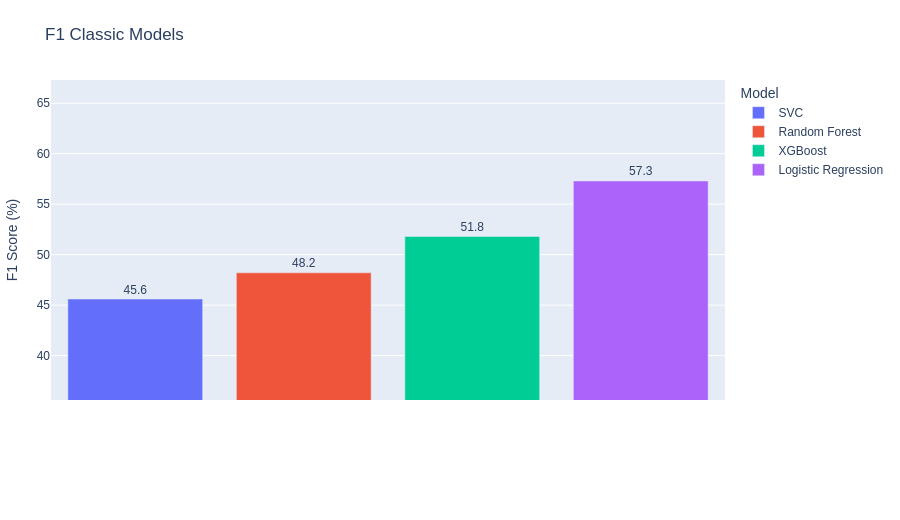
\includegraphics[width=1.0\linewidth]{images/F1-classic.png}
    \caption{Clásicos f1 score}
    \label{fig:Clasicos-f1-sore}
\end{figure}


\section{Transformers}
Para los transformers probados, todos han dado buenas respuestas. Todos los competidores conseguido superar en la validación al baseline, sin embargo, el que mejores resultados obtenido ha sido por parte de \textit{roberta-large-mnli}. 

El modelo de facebook deja detrás al resto con un $66.7$ f1 en validación,

\begin{figure}[H]
    \centering
    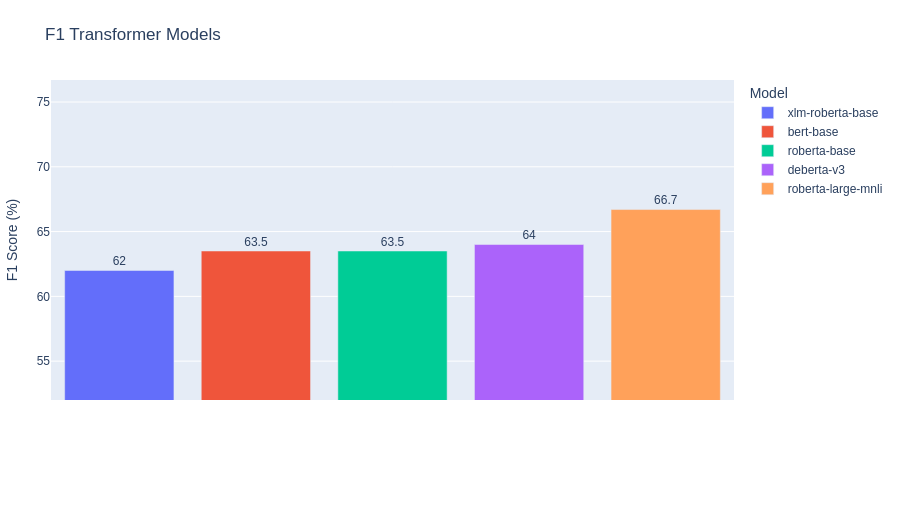
\includegraphics[width=1.0\linewidth]{images/F1-transformers.png}
    \caption{Transformers f1 score}
    \label{fig:Tranformers-f1-score}
\end{figure}


\section{LLMs}
Por último, tenemos a Gemini. Como se esperaba de él, ha roto todos los esquemas, consiguiendo en validación una puntuación de $83.4$ f1 en validación. Las capacidades de este modelo para tareas de este estilo se encuentra órdenes de magnitud por encima de los transformers clásicos. 

A cambio de un coste y tiempo de inferencia mucho más grande, conseguimos unos resultados de libro.

\begin{figure}[H]
    \centering
    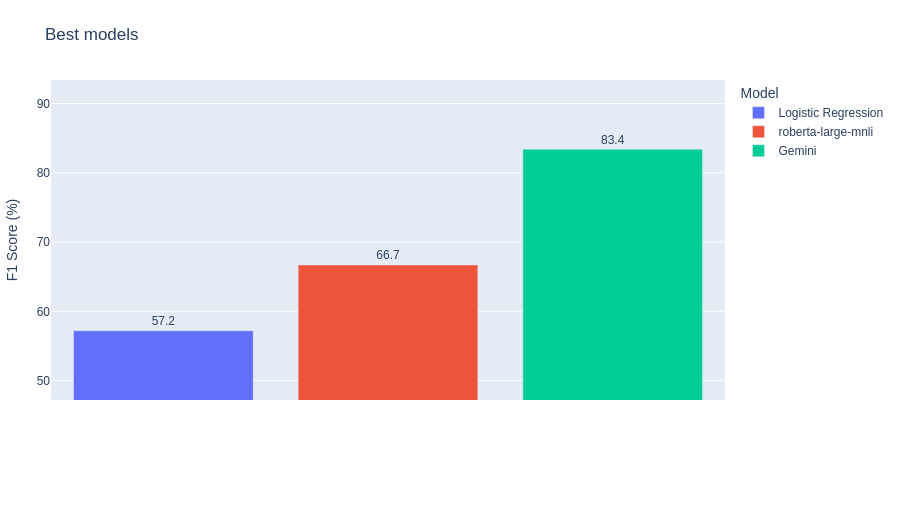
\includegraphics[width=1.0\linewidth]{images/F1-mejores.png}
    \caption{Mejores modelos}
    \label{fig:mores_modelos-f1-score}
\end{figure}

%%%%%%%%%%%%%%%%%%%%%%%%%%%%%%%%%%%%%%%%%%%%%%%%%%%%%%%%%%%%%%%%%%%%%%%%%%%%%%%
%                                 CONCLUSIONES                                 %
%%%%%%%%%%%%%%%%%%%%%%%%%%%%%%%%%%%%%%%%%%%%%%%%%%%%%%%%%%%%%%%%%%%%%%%%%%%%%%%
\chapter{Conclusiones}
Tras la realización de este trabajo, hemos probado formas de abordar la tarea de la clasificación multi-clase con modelos de tres distintas categorías. Todas, con sus ventajas y desventajas han mostrado defender su punto en las respuestas, proporcionando en mayor o menor medida soluciones buenas al problema.

En concreto, podemos ver que si NO disponemos de grandes capacidades computacionales, tendremos que conformarnos con el uso de modelos clásicos, como mejor opción Regresión logística. 

Por otro lado, si disponemos de GPUs de capacidad decente, podríamos atacar el problema mediante modelos más modernos como los transformers. Para esta tarea destacamos la arquitectura RoBERTa, en concreto la implementación de FaceBook: \textit{roberta-large-mnli}. 

Por último, si solo queremos los mejores resultados posibles en la tarea, nos da igual depender de servicios externos y el coste que tengan nuestras respuestas, deberemos ir con modelos de lenguaje tan grandes y capaces como podamos encontrar. Un ejemplo de estos es Gemini, con su versión \textit{gemini-2.5-pro}. 

%%%%%%%%%%%%%%%%%%%%%%%%%%%%%%%%%%%%%%%%%%%%%%%%%%%%%%%%%%%%%%%%%%%%%%%%%%%%%%%
%                                                                             %
%                                BIBLIOGRAFIA                                 %
%                                                                             %
%%%%%%%%%%%%%%%%%%%%%%%%%%%%%%%%%%%%%%%%%%%%%%%%%%%%%%%%%%%%%%%%%%%%%%%%%%%%%%%
\cleardoublepage
\printbibliography

%%%%%%%%%%%%%%%%%%%%%%%%%%%%%%%%%%%%%%%%%%%%%%%%%%%%%%%%%%%%%%%%%%%%%%%%%%%%%%%
%                                                                             %
%                                 APÉNDICESS                                  %
%                                                                             %
%%%%%%%%%%%%%%%%%%%%%%%%%%%%%%%%%%%%%%%%%%%%%%%%%%%%%%%%%%%%%%%%%%%%%%%%%%%%%%%

% \APPENDIX
%%%%%%%%%%%%%%%%%%%%%%%%%%%%%%%%%%%%%%%%%%%%%%%%%%%%%%%%%%%%%%%%%%%%%%%%%%%%%%%
%                        EJEMPLOS DE CADA TIPO DE FACTURA                     %
%%%%%%%%%%%%%%%%%%%%%%%%%%%%%%%%%%%%%%%%%%%%%%%%%%%%%%%%%%%%%%%%%%%%%%%%%%%%%%%

% \chapter{Apéndice ejemplo}
% \label{appendix:ejemplos}


%%%%%%%%%%%%%%%%%%%%%%%%%%%%%%%%%%%%%%%%%%%%%%%%%%%%%%%%%%%%%%%%%%%%%%%%%%%%%%%
%                              FIN DEL DOCUMENTO                              %
%%%%%%%%%%%%%%%%%%%%%%%%%%%%%%%%%%%%%%%%%%%%%%%%%%%%%%%%%%%%%%%%%%%%%%%%%%%%%%%
\end{document}
